% RLC-Parallelschwingkreis - Admittanzkurve |Y|/Bk von w/w0 mit Q=1,2,3,4,1000
\def\G{10e-3}%  10 mS
\def\L{10e-3}%  10 mH
\def\C{10e-6}%  10 uF
\def\Bk{31.623e-3}% Bk = sqrt(C/L) = 31.623 mS
% w0 = 1/sqrt(LC) = 3162.278 Hz
% Güte Q = Bk/G -> G = Bk/Q
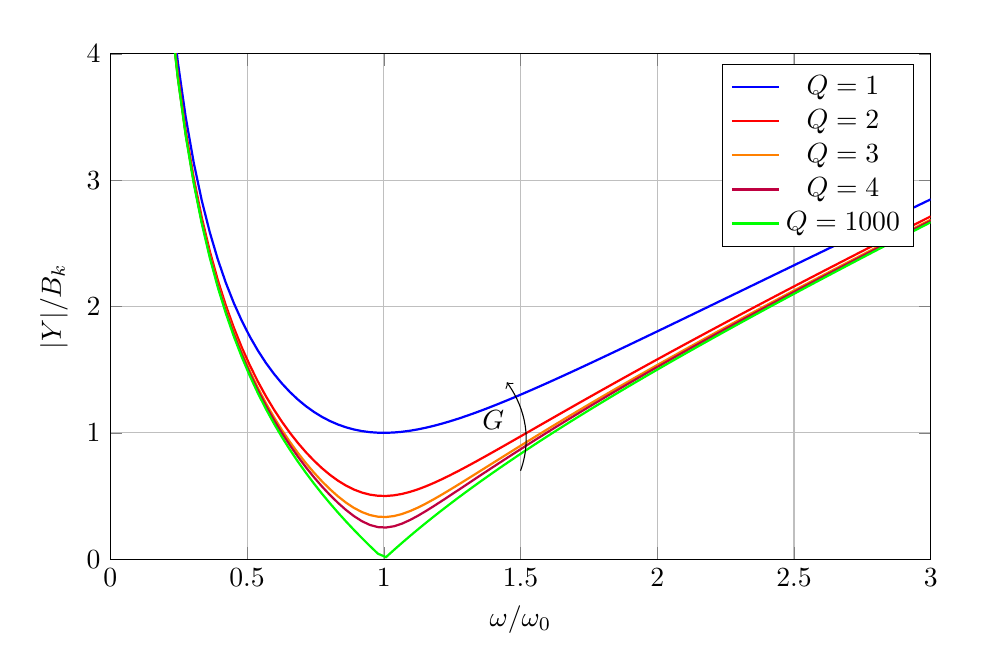
\begin{tikzpicture}[x=1cm,y=1cm]
    \draw[draw=none] (-1.05,-1) rectangle (10.75,6.75); % boundbox (not matching width and height, don't know why)
    \begin{axis}[
        xlabel={$\omega/\omega_0$},
        ylabel={$|Y|/B_k$},
        xmin=0, xmax=3,
        ymin=0, ymax=4,
        width=12cm,
        height=8cm,
        samples=100,
        grid=both,
        xtick={0, 0.5, 1, 1.5, 2, 2.5, 3},
    ]
    % Y/Bk = 1/Q + j(w/w0 - w0/w)
    % |Y|/Bk = sqrt( (1/Q)^2 + (w/w0 - w0/w)^2 )
    %\addplot[domain=0.1:3, mark=$Q=1$, thick, color=blue]     {sqrt((31.623e-3)^2+\Bk^2*(x-1/x)^2)/\Bk};     % Güte 1 -> G=31.623 mS -> R=31.62 Ohm
    %\addplot[domain=0.1:3, mark=$Q=2$, thick, color=red]      {sqrt((15.812e-3)^2+\Bk^2*(x-1/x)^2)/\Bk};     % Güte 2 -> G=15.812 mS -> R=15.81 Ohm
    %\addplot[domain=0.1:3, mark=$Q=3$, thick, color=orange]   {sqrt((10.541e-3)^2+\Bk^2*(x-1/x)^2)/\Bk};     % Güte 3 -> G=10.541 mS -> R=10.54 Ohm
    %\addplot[domain=0.1:3, mark=$Q=4$, thick, color=purple]   {sqrt((07.911e-3)^2+\Bk^2*(x-1/x)^2)/\Bk};     % Güte 4 -> G=7.911 mS -> R=7.91 Ohm
    %\addplot[domain=0.1:3, mark=$Q=1000$, thick, color=green] {sqrt((31.623e-6)^2+\Bk^2*(x-1/x)^2)/\Bk};  % Güte 1000 -> G=0.031623 mS -> R=0.032 Ohm
    \addplot[domain=0.1:3, mark=$Q=1$, thick, color=blue]     {sqrt((1/1)^2+(x-1/x)^2)};     % Güte 1 -> G=31.623 mS -> R=31.62 Ohm
    \addplot[domain=0.1:3, mark=$Q=2$, thick, color=red]      {sqrt((1/2)^2+(x-1/x)^2)};     % Güte 2 -> G=15.812 mS -> R=15.81 Ohm
    \addplot[domain=0.1:3, mark=$Q=3$, thick, color=orange]   {sqrt((1/3)^2+(x-1/x)^2)};     % Güte 3 -> G=10.541 mS -> R=10.54 Ohm
    \addplot[domain=0.1:3, mark=$Q=4$, thick, color=purple]   {sqrt((1/4)^2+(x-1/x)^2)};     % Güte 4 -> G=7.911 mS -> R=7.91 Ohm
    \addplot[domain=0.1:3, mark=$Q=1000$, thick, color=green] {sqrt((1/1000)^2+(x-1/x)^2)};  % Güte 1000 -> G=0.031623 mS -> R=0.032 Ohm
    \addlegendentry{$Q=1$}
    \addlegendentry{$Q=2$}
    \addlegendentry{$Q=3$}
    \addlegendentry{$Q=4$}
    \addlegendentry{$Q=1000$}
    % R Steigend 
    \draw [->](axis cs:1.5,0.7) .. controls (axis cs:1.55,1) and (axis cs:1.5, 1.25) .. (axis cs:1.45,1.4);
    \draw(axis cs:1.4, 1.1)node{$G$};
    \end{axis}
\end{tikzpicture}